\documentclass[11pt]{article}
\usepackage{graphicx}
\graphicspath{ {images/} }
\usepackage[margin=0.75in]{geometry}

\title{Reproducing fMRI Data Analysis on Brain Connectivity}
\author{
  Li, Jie\\
  \texttt{Jay4869}
  \and
  Li, Zeyu\\
  \texttt{lizeyuyuz}
  \and
  Yun, Chuan\\
  \texttt{ay2456}
  \and
  Zhang, Qingyuan\\
  \texttt{amandazhang}
}

\bibliographystyle{siam}

\begin{document}
\maketitle

\abstract{In this research paper, we attempt to reproduce fMRI data analysis
done by Repov and Barch in their paper exploring the relationship between
schizophrenia and brain connectivity \cite{repovs_barch1, repovs_barch2}. In
addition to the reproducing the ANOVA analysis of within and between brain
network connectivity, we analyze the given fMRI data using linear modeling,
time series as well as machine learning to explore various characteristics of
voxel behaviors in response to N-back tasks.}

\section{Introduction}

The paper of which our research is based is titled ``Working memory related
brain network connectivity in individuals with schizophrenia and their
siblings'' \cite{repovs_barch1, repovs_barch2}. Schizophrenia is a chronic,
severe, and disabling brain disorder. Previous studies have shown that changes
in the function of a single brain region, or even a brain system, cannot
explain the functional impairments seen in this illness \ \cite{repovs_barch1}.
However, Repovs and Barch attempts to show that individuals with schizophrenia
have reduced connectivity within and between neural networks, which could be a
forward step to understanding schizophrenia. \par

In their paper, the writers try to systematically examine changes in functional
connectivity across rest and different task states in order to make an
inference on characteristics of schizophrenia. The authors found four types of
participates, individuals with schizophrenia, the siblings of individuals with
schizophrenia, healthy controls and the siblings of healthy controls. They
designed three working memory loads of an N-back task and designated four
regions of interest (ROIs). The four brain networks are: (1) Dorsal
fronto-parietal network (FP), (2) Cingulo-opercular network (CO), (3)
Cerebellar network (CER) and (4) "Default mode" network (DMN). The objective of
the study is to examine the altered functional connectivity within and between
these four brain networks when the participant performing a designated N-back
task. After analyzing the data using ANOVA, the authors found that that
individuals with schizophrenia and their siblings showed consistent reductions
in connectivity between both the FP and CO networks with the CER network. \par

In our attempt to reproduce the analysis done by Repovs and Barch, we first
examine the validity of their use of ANOVA methods to assess functional
connectivity. On top of that, we will make necessary simplifications and model
the data using various analysis methods such as linear modeling, time series,
as well as machine learning. \par
%You should explain the basic idea of the paper in a paragraph.  You should also perform basic sanity check on the data
%(e.g., can you downloaded, can you load the files, confirm that you have the correct number of subjects).
%Briefly explain what reproducibility means and in what sense you will try to reproduce this study.

\section{Data}
\paragraph{}
The data used in their published paper is available on the website
OpenFMRI.org. The are many data files grouped by subjects, but we will be
focusing on only a few subjects due to time and resource constraints. We start
off analyzing a single subject, subject 001, who is male, Caucasian and
Schizophrenic. If we have time, we will extend our analysis on comparing two
subjects, one with schizophrenia and one healthy control. Each subject contains
four folders, and for our analysis, we focus on the folder containing blood
oxygen level dependent (BOLD) time series. \par
We went to OpenFMRI.org and looked through all the files it has for this paper. 
The are many data files grouped by subjects and we only downloaded 
``ds115-sub001-005.tg'', which contains the brain image of the first five 
subjects, and the ``ds115-metadata.tg'', which contains metadata for the paper.
Since we only chose one subject, which is sub001, we only need his part in the
data file.\par 
First, we checked all the files for sub001 and found there are three tasks for 
our subject. We realized that these were ``N - back'' working memory task in 
the paper. This task was to respond for each letter shown whether it was the 
same as a pre-specified letter (0-back), the same as the immediately preceding 
letter (1-back), or the same as the letter shown two trials previously (2-back).
For our subject, there were three BOLD runs, each consisting of two blocks of 
0-back, 1-back, or 2-back working memory task. \par
Second, we found that under each task there are four brain images. We thought 
one of them should be the raw image and the others were some-how processed by 
the authors. Therefore, we plotted these four brain images and chose the most 
blurred one (This is probably because it is after smoothing), which is
``BOLD-mcf-brain.nii''.\par
Then, similar to what we did in class, we used HRF function to convolve our 
neural prediction, This will give us a hemodynamic prediction, under the 
linear-time-invariant assumptions of the convolution. This is a very important 
step because we will use convolution data in our linear modeling process in the
future. Here is the comparison between the original neural prediction and 
convolved.

\begin{figure}[!htb]
    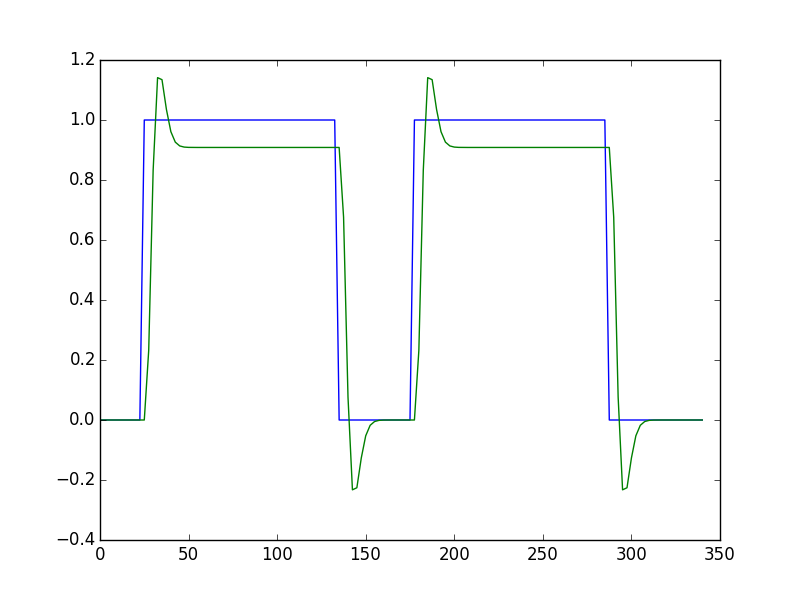
\includegraphics[width=\linewidth]{task001_run001_conv005}
\end{figure}

\section{Methods}
\subsection{Linear Modeling}
\paragraph{}
First of all, we did a muti-variables linear regression on convolving response 
(design matrix $X$) and blood pressure(response $Y$). We constructed the design 
matrix $X$, which dimension is (133, 2) and reshaped our blood pressure data from 
4 dimension to 2 dimension.\par
Second, under the assumption of constant variance and normality of our data, we 
use OLS method to calculate $\hat{\beta}$, the formula is 
$\hat{\beta_{ls}}=(X^{T}X)^{-1}X^{T}Y$. We plug in $X$ and $Y$ to get
our $\hat{\beta_{ls}}$, which is a 2 by 147456 matrix. Then we reshaped it into 
4 dimension. Based on the $\hat{\beta_{ls}}$ we got from muti-variables linear 
regression, we compute the fitted value $\hat{Y}$, which equals 
$X\hat{\beta_{ls}}$. The residual $\hat{e}$, which equals $Y-\hat{Y}$. The 
residual sum of squares $RSS$, which is $\hat{e}^{T}\hat{e}$. The covariance
matrix of $\hat{\beta_{ls}}$ is $cov(\beta_{ls}) = \sigma^2(X^{T}X)^{-1}$. Here $\sigma^2$
is unknown, we use $\hat{\sigma}^2 = \frac{RSS}{n-r}$, which is an unbiased 
estimate of $\sigma^2$. Thus the covariance matrix 
$cov(\beta_{ls}) = \frac{RSS}{n-r}(X^{T}X)^{-1}$. \par
Then, we generated our null hypothesis test:$\hat{\beta} = 0$.\par
By using t-test and set our significance level as 10\%, we found there are 1507 
out of 147456 voxels that have the significant effect between our task and 
blood pressure, so we defined the sub-area of brain contains the most 
significant voxels by plotting a p-value map.

\section{Results}
\begin{figure}[!htb]
  \centering
  \begin{minipage}[b]{0.4\textwidth}
    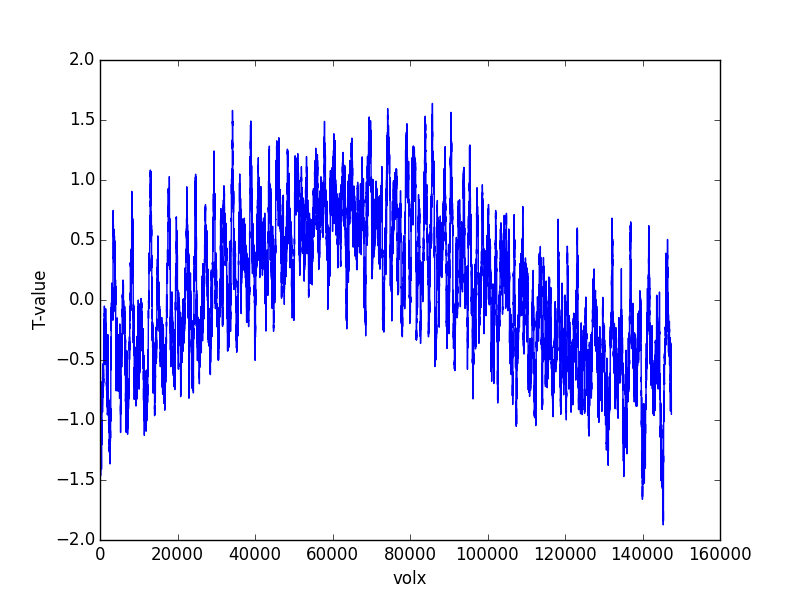
\includegraphics[width=\textwidth]{T_value}
    \caption{Plot of T values.}
  \end{minipage}
  \hfill
  \begin{minipage}[b]{0.4\textwidth}
    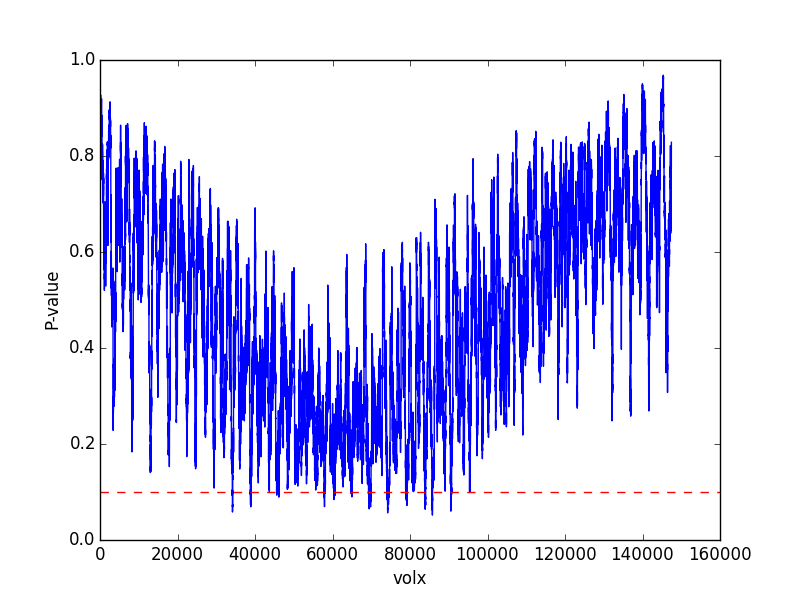
\includegraphics[width=\textwidth]{p_value}
    \caption{Plot of P values.}
  \end{minipage}
\end{figure}
\subsection{Data Preprocessing}
\paragraph{}
First, we checked all the files for sub001 and found there are three tasks for
our subject. We realized that these were ``N - back'' working memory task in
the paper. This task was to respond for each letter shown whether it was the
same as a pre-specified letter (0-back), the same as the immediately preceding
letter (1-back), or the same as the letter shown two trials previously
(2-back). For our subject, there were three BOLD runs, each consisting of two
blocks of 0-back, 1-back, or 2-back working memory task. 

Second, we found that under each task there are four brain images. We thought
one of them should be the raw image and the others were some-how processed by
the authors. Therefore, we plotted these four brain images and chose the most
blurred one (This is probably because it is after smoothing), which is
``BOLD-mcf-brain.nii''. 

Then, similar to what we did in class, we used HRF function to convolve our
neural prediction, This will give us a hemodynamic prediction, under the
linear-time-invariant assumptions of the convolution. This is a very important
step because we will use convolution data in our linear modeling process in the
future. Here is the comparison between the original neural prediction and
convolved.

\section{Discussion}
\subsection{Obstacles} 

The hardest part of the project is understanding which direction we should go
given the time constraint and limited knowledge on the subject. 

\bibliography{report}

\end{document}
